\documentclass{standalone}
\usepackage{tikz}
\usetikzlibrary{patterns}
\usetikzlibrary{positioning}
\usetikzlibrary{patterns, positioning}
\usetikzlibrary{shapes.misc}
\usepackage[outline]{contour}
\contourlength{1.5pt} 
\usepackage[sfdefault]{ClearSans}

\begin{document}
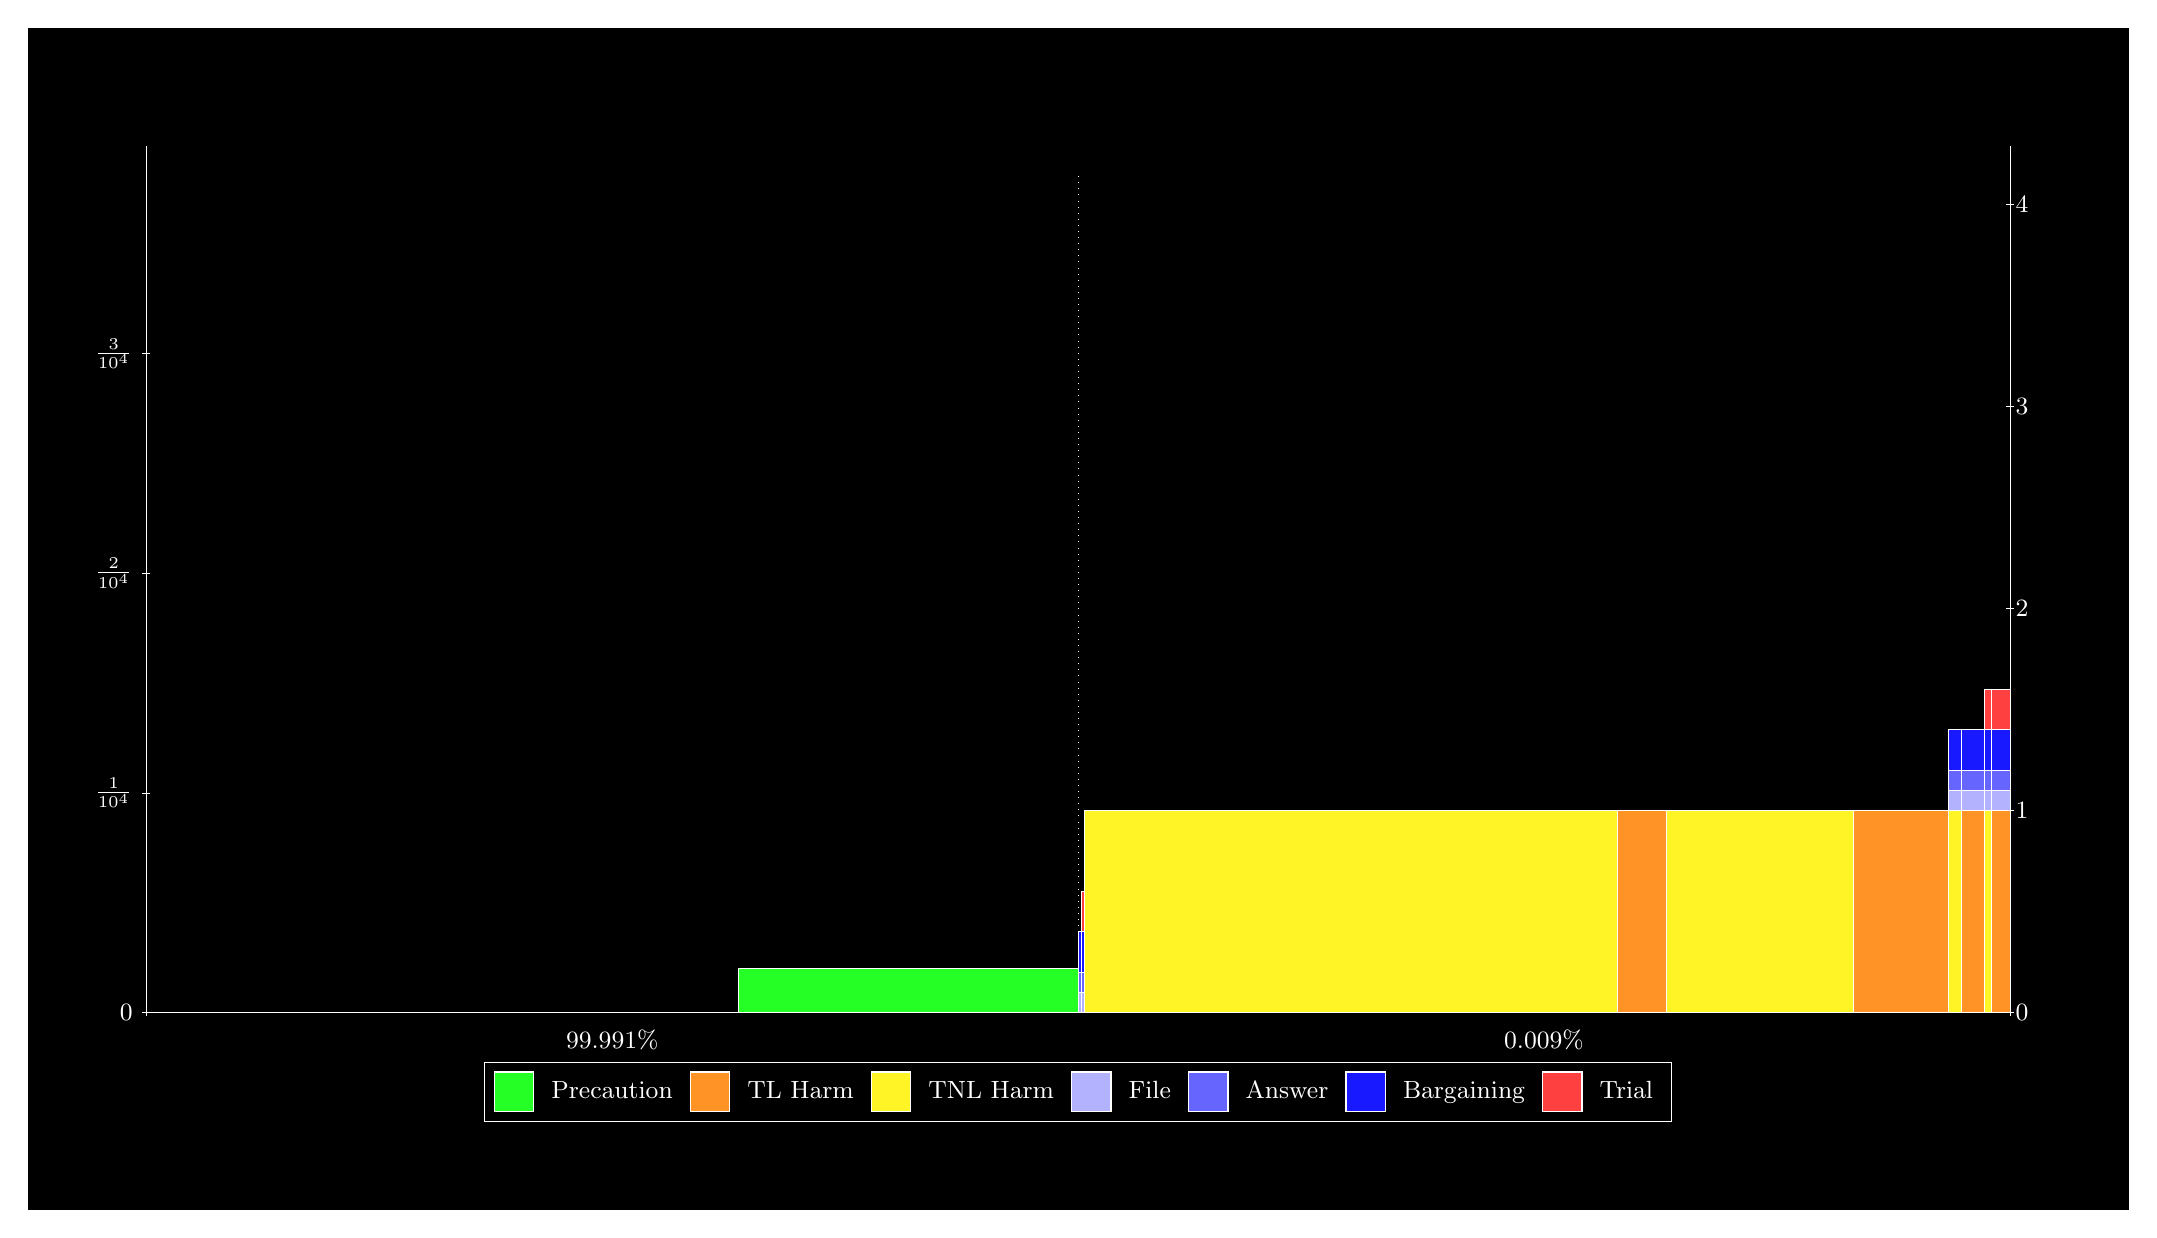
\begin{tikzpicture}
\draw[fill=black] (0,0) rectangle (26.667,15);
\draw[fill=green!85,draw=white,very thin] (9.0126,2.5) rectangle (13.333,3.0579);
\draw[fill=blue!30,draw=white,very thin] (13.333,2.5) rectangle (13.379,2.7565);
\draw[fill=blue!60,draw=white,very thin] (13.333,2.7565) rectangle (13.379,3.0129);
\draw[fill=blue!90,draw=white,very thin] (13.333,3.0129) rectangle (13.379,3.5259);
\draw[fill=blue!30,draw=white,very thin] (13.379,2.5) rectangle (13.412,2.7565);
\draw[fill=blue!60,draw=white,very thin] (13.379,2.7565) rectangle (13.412,3.0129);
\draw[fill=blue!90,draw=white,very thin] (13.379,3.0129) rectangle (13.412,3.5259);
\draw[fill=red!75,draw=white,very thin] (13.379,3.5259) rectangle (13.412,4.0388);
\draw[fill=yellow!85,draw=white,very thin] (13.412,2.5) rectangle (20.181,5.0647);
\draw[fill=orange!85,draw=white,very thin] (20.181,2.5) rectangle (20.802,5.0647);
\draw[fill=green!85,draw=white,very thin] (20.802,2.5) rectangle (23.181,2.5001);
\draw[fill=yellow!85,draw=white,very thin] (20.802,2.5001) rectangle (23.181,5.0647);
\draw[fill=green!85,draw=white,very thin] (23.181,2.5) rectangle (24.385,2.5001);
\draw[fill=orange!85,draw=white,very thin] (23.181,2.5001) rectangle (24.385,5.0647);
\draw[fill=yellow!85,draw=white,very thin] (24.385,2.5) rectangle (24.546,5.0647);
\draw[fill=blue!30,draw=white,very thin] (24.385,5.0647) rectangle (24.546,5.3212);
\draw[fill=blue!60,draw=white,very thin] (24.385,5.3212) rectangle (24.546,5.5776);
\draw[fill=blue!90,draw=white,very thin] (24.385,5.5776) rectangle (24.546,6.0906);
\draw[fill=orange!85,draw=white,very thin] (24.546,2.5) rectangle (24.838,5.0647);
\draw[fill=blue!30,draw=white,very thin] (24.546,5.0647) rectangle (24.838,5.3212);
\draw[fill=blue!60,draw=white,very thin] (24.546,5.3212) rectangle (24.838,5.5776);
\draw[fill=blue!90,draw=white,very thin] (24.546,5.5776) rectangle (24.838,6.0906);
\draw[fill=yellow!85,draw=white,very thin] (24.838,2.5) rectangle (24.931,5.0647);
\draw[fill=blue!30,draw=white,very thin] (24.838,5.0647) rectangle (24.931,5.3212);
\draw[fill=blue!60,draw=white,very thin] (24.838,5.3212) rectangle (24.931,5.5776);
\draw[fill=blue!90,draw=white,very thin] (24.838,5.5776) rectangle (24.931,6.0906);
\draw[fill=red!75,draw=white,very thin] (24.838,6.0906) rectangle (24.931,6.6035);
\draw[fill=orange!85,draw=white,very thin] (24.931,2.5) rectangle (25.167,5.0647);
\draw[fill=blue!30,draw=white,very thin] (24.931,5.0647) rectangle (25.167,5.3212);
\draw[fill=blue!60,draw=white,very thin] (24.931,5.3212) rectangle (25.167,5.5776);
\draw[fill=blue!90,draw=white,very thin] (24.931,5.5776) rectangle (25.167,6.0906);
\draw[fill=red!75,draw=white,very thin] (24.931,6.0906) rectangle (25.167,6.6035);
\draw[white,very thin] (1.5,2.5) -- (1.5,13.5);
\draw[white,very thin] (1.45,2.5) -- (1.55,2.5);
\node[font=\small,text=white, anchor=east] at (1.45, 2.5) {0};
\draw[white,very thin] (1.45,5.2896) -- (1.55,5.2896);
\node[font=\small,text=white, anchor=east] at (1.45, 5.2896) {$\frac{1}{10^{4}}$};
\draw[white,very thin] (1.45,8.0792) -- (1.55,8.0792);
\node[font=\small,text=white, anchor=east] at (1.45, 8.0792) {$\frac{2}{10^{4}}$};
\draw[white,very thin] (1.45,10.869) -- (1.55,10.869);
\node[font=\small,text=white, anchor=east] at (1.45, 10.869) {$\frac{3}{10^{4}}$};

\draw[white,dotted,very thin] (13.333,2.83) -- (13.333,13.17);
\draw[white,very thin] (25.167,2.5) -- (25.167,13.5);
\draw[white,very thin] (25.117,2.5) -- (25.217,2.5);
\node[font=\small,text=white, anchor=west] at (25.117, 2.5) {0};
\draw[white,very thin] (25.117,5.0647) -- (25.217,5.0647);
\node[font=\small,text=white, anchor=west] at (25.117, 5.0647) {1};
\draw[white,very thin] (25.117,7.6294) -- (25.217,7.6294);
\node[font=\small,text=white, anchor=west] at (25.117, 7.6294) {2};
\draw[white,very thin] (25.117,10.194) -- (25.217,10.194);
\node[font=\small,text=white, anchor=west] at (25.117, 10.194) {3};
\draw[white,very thin] (25.117,12.759) -- (25.217,12.759);
\node[font=\small,text=white, anchor=west] at (25.117, 12.759) {4};

\draw[white,very thin] (1.5,2.5) -- (25.167,2.5);
\draw[white,very thin] (1.5,2.45) -- (1.5,2.55);
\node[font=\small,text=white, anchor=north] at (1.5, 2.45) {};
\draw[white,very thin] (25.167,2.45) -- (25.167,2.55);
\node[font=\small,text=white, anchor=north] at (25.167, 2.45) {};

\node[font=\small,text=white,anchor=south] at (7.4167, 1.9) {99.991\%};
\node[font=\small,text=white,anchor=south] at (19.25, 1.9) {0.009\%};
\draw (13.3333,2.5) node (B) {};
\begin{scope}[align=center]
\matrix[scale=0.5,draw=white,below=0.5cm of B,nodes={draw},column sep=0.1cm]{
\node[rectangle,draw,minimum width=0.5cm,minimum height=0.5cm,fill=green!85]{}; & \node[draw=none,font=\small,text=white]{Precaution}; &
\node[rectangle,draw,minimum width=0.5cm,minimum height=0.5cm,fill=orange!85]{}; & \node[draw=none,font=\small,text=white]{TL Harm}; &
\node[rectangle,draw,minimum width=0.5cm,minimum height=0.5cm,fill=yellow!85]{}; & \node[draw=none,font=\small,text=white]{TNL Harm}; &
\node[rectangle,draw,minimum width=0.5cm,minimum height=0.5cm,fill=blue!30]{}; & \node[draw=none,font=\small,text=white]{File}; &
\node[rectangle,draw,minimum width=0.5cm,minimum height=0.5cm,fill=blue!60]{}; & \node[draw=none,font=\small,text=white]{Answer}; &
\node[rectangle,draw,minimum width=0.5cm,minimum height=0.5cm,fill=blue!90]{}; & \node[draw=none,font=\small,text=white]{Bargaining}; &
\node[rectangle,draw,minimum width=0.5cm,minimum height=0.5cm,fill=red!75]{}; & \node[draw=none,font=\small,text=white]{Trial}; \\\\
};\end{scope}

\end{tikzpicture}
\end{document}